%META {"question":"Hai tia Ox và Oy trong hình có là hai tia đối nhau không?","options":["Không — vì Ox và Oy không cùng nằm trên một đường thẳng","Có — vì chúng chung gốc O","Có — vì góc xOy bé hơn 180°","Không thể xác định"],"answer":0,"note":"Tia đối yêu cầu: chung gốc VÀ cùng nằm trên một đường thẳng. Ở đây góc xOy nhọn hơn 180° nên không phải tia đối."}
\documentclass[border=5pt]{standalone}
\usepackage{tkz-euclide}
% Màu dùng chung cho toàn bộ hình vẽ (ảnh stack với nền tối của web)
\definecolor{tminc}{RGB}{226,232,240}   % chữ + nét chính
\definecolor{tmblue}{RGB}{0,210,255}    % nhấn neon xanh
\definecolor{tmpink}{RGB}{255,0,200}    % nhấn neon hồng
\definecolor{tmgreen}{RGB}{0,255,136}   % nhấn neon xanh lá
\color{tminc}

\begin{document}
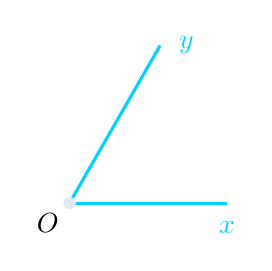
\begin{tikzpicture}[line width=1.1pt]
  \coordinate (O) at (0,0);
  \coordinate (X) at (2,0);
  \coordinate (Y) at (1.15,2);
  \draw[tmblue] (O) -- (X) node[below=3pt]{$x$};
  \draw[tmblue] (O) -- (Y) node[right=3pt]{$y$};
  \tkzDrawPoints[size=3.5,color=tminc,fill=tminc](O)
  \tkzLabelPoint[below left](O){$O$}
\end{tikzpicture}
\end{document}
